\documentclass[aspectratio=169, table]{beamer}


%\usepackage[beamertheme=./praditatheme]{Pradita}

\graphicspath{{../../images/}}

\usetheme{Pradita}

\subtitle{IF231303-Software Architecture  \vspace{10pt}}
\title{\huge Chapter-8:\\Serverless Architecture}
\author{\textbf{Yogi Valentino N, Steven Tanaka, Ryan Christensen\\Alfa Yohannis}}

\begin{document}

    \begin{frame}[plain]
        \maketitle
    \end{frame}

    \begin{frame}
        \frametitle{Definisi Serverless Architecture}
        %		\framesubtitle{\hspace{1cm}}
        \begin{itemize}
            \item \emph{Serverless architecture} merupakan pendekatan dalam desain \emph{software} yang mana developer tidak perlu lagi direpotkan mengelola infrastruktur seperti server.
            \item Developer bisa fokus dalam mengembangkan aplikasinya dan masalah server akan dikelola oleh penyedia layanan \emph{serverless} (provider).
            \item \emph{Serverless architecture} bukan berarti tanpa server sama sekali, tetapi memungkinkan untuk konfigurasi seminimal mungkin atau dikurangi.
        \end{itemize}
    \end{frame}

    \begin{frame}
        \centering
        \begin{figure}
            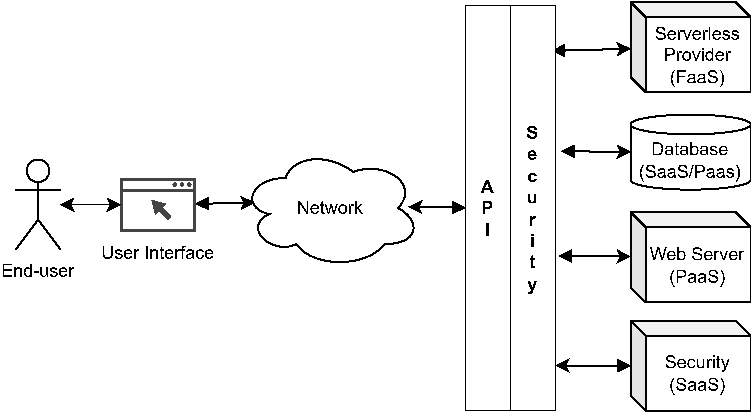
\includegraphics[width=\linewidth]{serverless_architecture}
            \caption{Components of Serverless Architecture}
        \end{figure}
    \end{frame}

    \begin{frame}
        \frametitle{6 Key Components of Serverless Architecture:}
        \framesubtitle{1. Function as a Service (FaaS)}
        \begin{itemize}
            \item
            FaaS adalah blok bangunan dasar dari serverless, bertanggung jawab untuk menjalankan logika yang menentukan bagaimana sumber daya dialokasikan dalam suatu skenario tertentu.
            \item Tergantung pada lingkungan cloud yang digunakan, pengguna dapat memilih layanan FaaS yang dirancang khusus seperti AWS Lambda untuk Amazon Web Services (AWS), Microsoft Azure Functions untuk Azure, Google Cloud Functions untuk Google Cloud Platform (GCP), dan IBM Cloud Functions
            \item Fungsi-fungsi ini akan membaca menerima data dari pengguna ketika suatu peristiwa terjadi dan memproses serta mengirimkan balik hasil.
        \end{itemize}
    \end{frame}

    \begin{frame}
        \frametitle{6 Key Components of Serverless Architecture:}
        \framesubtitle{2. The Client Interface}
        \begin{itemize}
            \item
            Antarmuka klien memainkan peran penting dalam fungsionalitas serverless.
            \item Antarmuka harus mampu mendukung serangkaian permintaan (dengan waktu tunggu) yang singkat and interaksi tanpa keadaan (\textit{stateless}).
            \item Antarmuka juga harus dirancang agar kompatibel dengan transfer data, baik dalam volume yang sangat tinggi maupun rendah.
        \end{itemize}
    \end{frame}

    \begin{frame}\frametitle{6 Key Components of Serverless Architecture:}
        \framesubtitle{3. A web server on the Cloud}
        \vspace{20pt}
        \begin{itemize}
            \item Server web adalah tempat interaksi tanpa keadaan (\textit{stateless}) akan dimulai setelah pengguna memulainya dan sampai layanan FaaS menghentikannya (umumnya karena hasil komputasi telah dikembalikan).
            \item Server web berbeda dari \textit{database backend}, di mana informasi yang dikirimkan kepada pengguna disimpan. Misalnya, konten gambar.
            \item Server web, dalam hal ini, hanya menyimpan  permintaan pengguna, data/gambar kiriman dari pengguna yang untuk diproses, hasil komputasi, sebelum keseluruhan proses dihentikan sesuai dengan sifat sementara dari serverless.
            \item Konten gambar yang telah diproses dan dikembalikan akan disimpan di penyimpanan backend, menunggu untuk diambil sesuai permintaan pengguna.
        \end{itemize}
    \end{frame}

    \begin{frame}\frametitle{6 Key Components of Serverless Architecture:}
        \framesubtitle{4. A Security Service}
        \vspace{20pt}
        Keamanan adalah elemen kunci dari operasi serverless karena:
        \begin{itemize}
            \item Aplikasi menangani ribuan permintaan secara bersamaan. Setiap permintaan harus diotentikasi sebelum mengirimkan respons.
            \item Karena sifatnya yang \textit{stateless}, riwayat interaksi sebelumnya tidak disimpan. Aplikasi tidak dapat mengandalkan interaksi sebelumnya untuk memvalidasi interaksi di masa depan.
            \item Model serverless membuat transparansi dan pemantauan menjadi lebih sulit. Sistem harus mendapatkan informasi keamanan dari jutaan peristiwa yang dicatat setiap hari.
            \item Sifat terdistribusi dari arsitektur \textit{serverless} berarti ada beberapa layanan dan vendor yang terlibat, dan semuanya harus diamankan.
        \end{itemize}
    \end{frame}

    \begin{frame}\frametitle{6 Key Components of Serverless Architecture:}
        \framesubtitle{4. A Security Service}
        \vspace{20pt}
        Keamanan adalah elemen kunci dari operasi serverless karena:
        \begin{itemize}
            \item Biasanya, aplikasi serverless menggunakan layanan token, di mana kredensial sementara dihasilkan untuk pengguna dan dapat digunakan untuk memanggil fungsi.
            \item Sistem serverless juga dapat diintegrasikan dengan layanan manajemen identitas dan akses yang siap digunakan dengan serverless ke dalam aplikasi. Sebagai contoh, AWS Cognito bekerja dengan AWS Lambda untuk mengautentikasi identitas pengguna melalui SSO atau jaringan sosial.
        \end{itemize}
    \end{frame}


    \begin{frame}\frametitle{6 Key Components of Serverless Architecture: }
        \framesubtitle{5. Database Backend}
        \begin{itemize}
            \item Database backend adalah tempat data disimpan.
            \item Database backend juga bertanggung jawab untuk mengelola data yang dikirimkan oleh pengguna.
            \item Ini adalah komponen yang paling penting dari arsitektur serverless karena menyimpan dan mengolah informasi yang dikirimkan dari dan kepada pengguna.
        \end{itemize}
    \end{frame}

    \begin{frame}\frametitle{6 Key Components of Serverless Architecture:}
        \framesubtitle{6. API Gateway}
        \begin{itemize}
            \item API Gateway bertindak sebagai gerbang untuk menghubungkan pengguna dengan fungsi yang sesuai.
            \item Ini adalah komponen yang sangat penting dari arsitektur serverless karena memungkinkan Anda untuk mengontrol lalu lintas dan memastikan bahwa permintaan yang masuk diteruskan ke fungsi yang sesuai.
            \item API Gateway juga memungkinkan sistem serverless untuk mengatur kebijakan akses dan otentikasi untuk memastikan bahwa pengguna yang sah dapat mengakses fungsi yang sesuai.
        \end{itemize}
    \end{frame}

    \begin{frame}\frametitle{Serverless Architecture}
        %		\framesubtitle{\hspace{1cm}}
        Dalam keseluruhan arsitektur serverless:
        \begin{itemize}
            \item FaaS berperan sebagai eksekutor logika yang menentukan alokasi sumber daya,
            \item antarmuka klien berfungsi sebagai antarmuka pengguna,
            \item server web di cloud menangani interaksi tanpa keadaan,
            \item layanan keamanan menjaga keamanan dan otentikasi,
            \item database backend menyimpan data yang akan dikirimkan kepada pengguna, dan
            \item API gateway menghubungkan semua komponen tersebut.
        \end{itemize}
    \end{frame}


    \begin{frame}\frametitle{Manfaat Serverless Architecture}
        %		\framesubtitle{\hspace{1cm}}
        \vspace{20pt}
        Beberapa keuntungan dari penggunaan arsitektur serverless:
        \begin{itemize}
            \item \textbf{Optimasi Biaya}. optimisasi biaya dengan hanya membayar untuk sumber daya yang digunakan
            \item memungkinkan pengembangan aplikasi yang lebih cepat
            \item \textbf{Skalabilitas}. skalabilitas yang mudah untuk mengakomodasi perubahan permintaan
            \item \textbf{Perawatan}. serta perawatan dan pemeliharaan yang lebih mudah karena dikelola oleh penyedia layanan awan.
            \item \textbf{Fokus pada pengembangan aplikasi}. Dalam serverless, pengembang tidak perlu khawatir mengurus infrastruktur server dan dapat fokus pada pengembangan aplikasi.
        \end{itemize}
    \end{frame}

    \begin{frame}\frametitle{Kekurangan Serverless Architecture}
        \framesubtitle{\hspace{1cm}}
        \vspace{20pt}
        \begin{itemize}
            \item \textbf{Keterbatasan Pengaturan.} Tidak cocok untuk semua jenis aplikasi, terutama jika aplikasi memerlukan kontrol tinggi atas infrastruktur dan lingkungan di mana aplikasi berjalan.
            \item \textbf{Ketergantungan.} Bergantung pada penyedia layanan awan, sehingga jika terjadi masalah atau gangguan pada layanan, aplikasi dapat mengalami \textit{downtime} yang signifikan.
            \item \textbf{Pengaturan konfigurasi kompleks. } Memiliki konfigurasi yang kompleks dan memerlukan pengaturan yang cermat untuk memastikan aplikasi berjalan dengan baik.
            \item \textbf{Performa dapat tidak stabil.} Performa dapat tidak stabil jika karena bergantung pada pihak penyedia layanan.
        \end{itemize}
    \end{frame}


    \begin{frame}\frametitle{Penerapan Serverless Architecture}
        %		\framesubtitle{\hspace{1cm}}
        \begin{itemize}
            \item \textbf{Web applications.} Pengembang dapat membangun dan menerapkan aplikasi web menggunakan arsitektur tanpa server, tanpa harus mengelola server atau infrastruktur.
            \item \textbf{Data processing.} Serverless Architecture dapat digunakan untuk tugas pemrosesan data seperti transformasi data, pembersihan, dan analisis tanpa harus mengelola server atau infrastruktur.
            \item Aplikasi lainnya yang tidak memerlukan pengelolaan server mandiri.

        \end{itemize}
    \end{frame}


%    \begin{frame}\frametitle{Penerapan Serverless Architecture (2)}
%        \framesubtitle{\hspace{1cm}}
%        \begin{itemize}
%            \item \textbf{Chatbots:} Pengembang dapat membangun chatbot menggunakan serverless, dengan menulis kode yang merespons acara obrolan, seperti pesan pengguna. Mereka dapat menggunakan layanan seperti AWS Lex, Google Cloud Dialogflow, atau Azure Bot Service untuk membuat dan menerapkan chatbot yang berjalan sesuai permintaan.
%            \item \textbf {IoT applications:} Serverless Architecture dapat digunakan untuk aplikasi IoT, dengan memungkinkan pengembang menulis kode yang merespons kejadian dari perangkat IoT, seperti pembacaan sensor. Mereka dapat menggunakan layanan seperti AWS IoT, Google Cloud IoT Core, atau Azure IoT Hub untuk membangun dan menerapkan aplikasi IoT tanpa server.
%        \end{itemize}
%    \end{frame}
\end{document}